\documentclass{article}
\usepackage{tikz}
\usetikzlibrary{arrows.meta, positioning}

\begin{document}

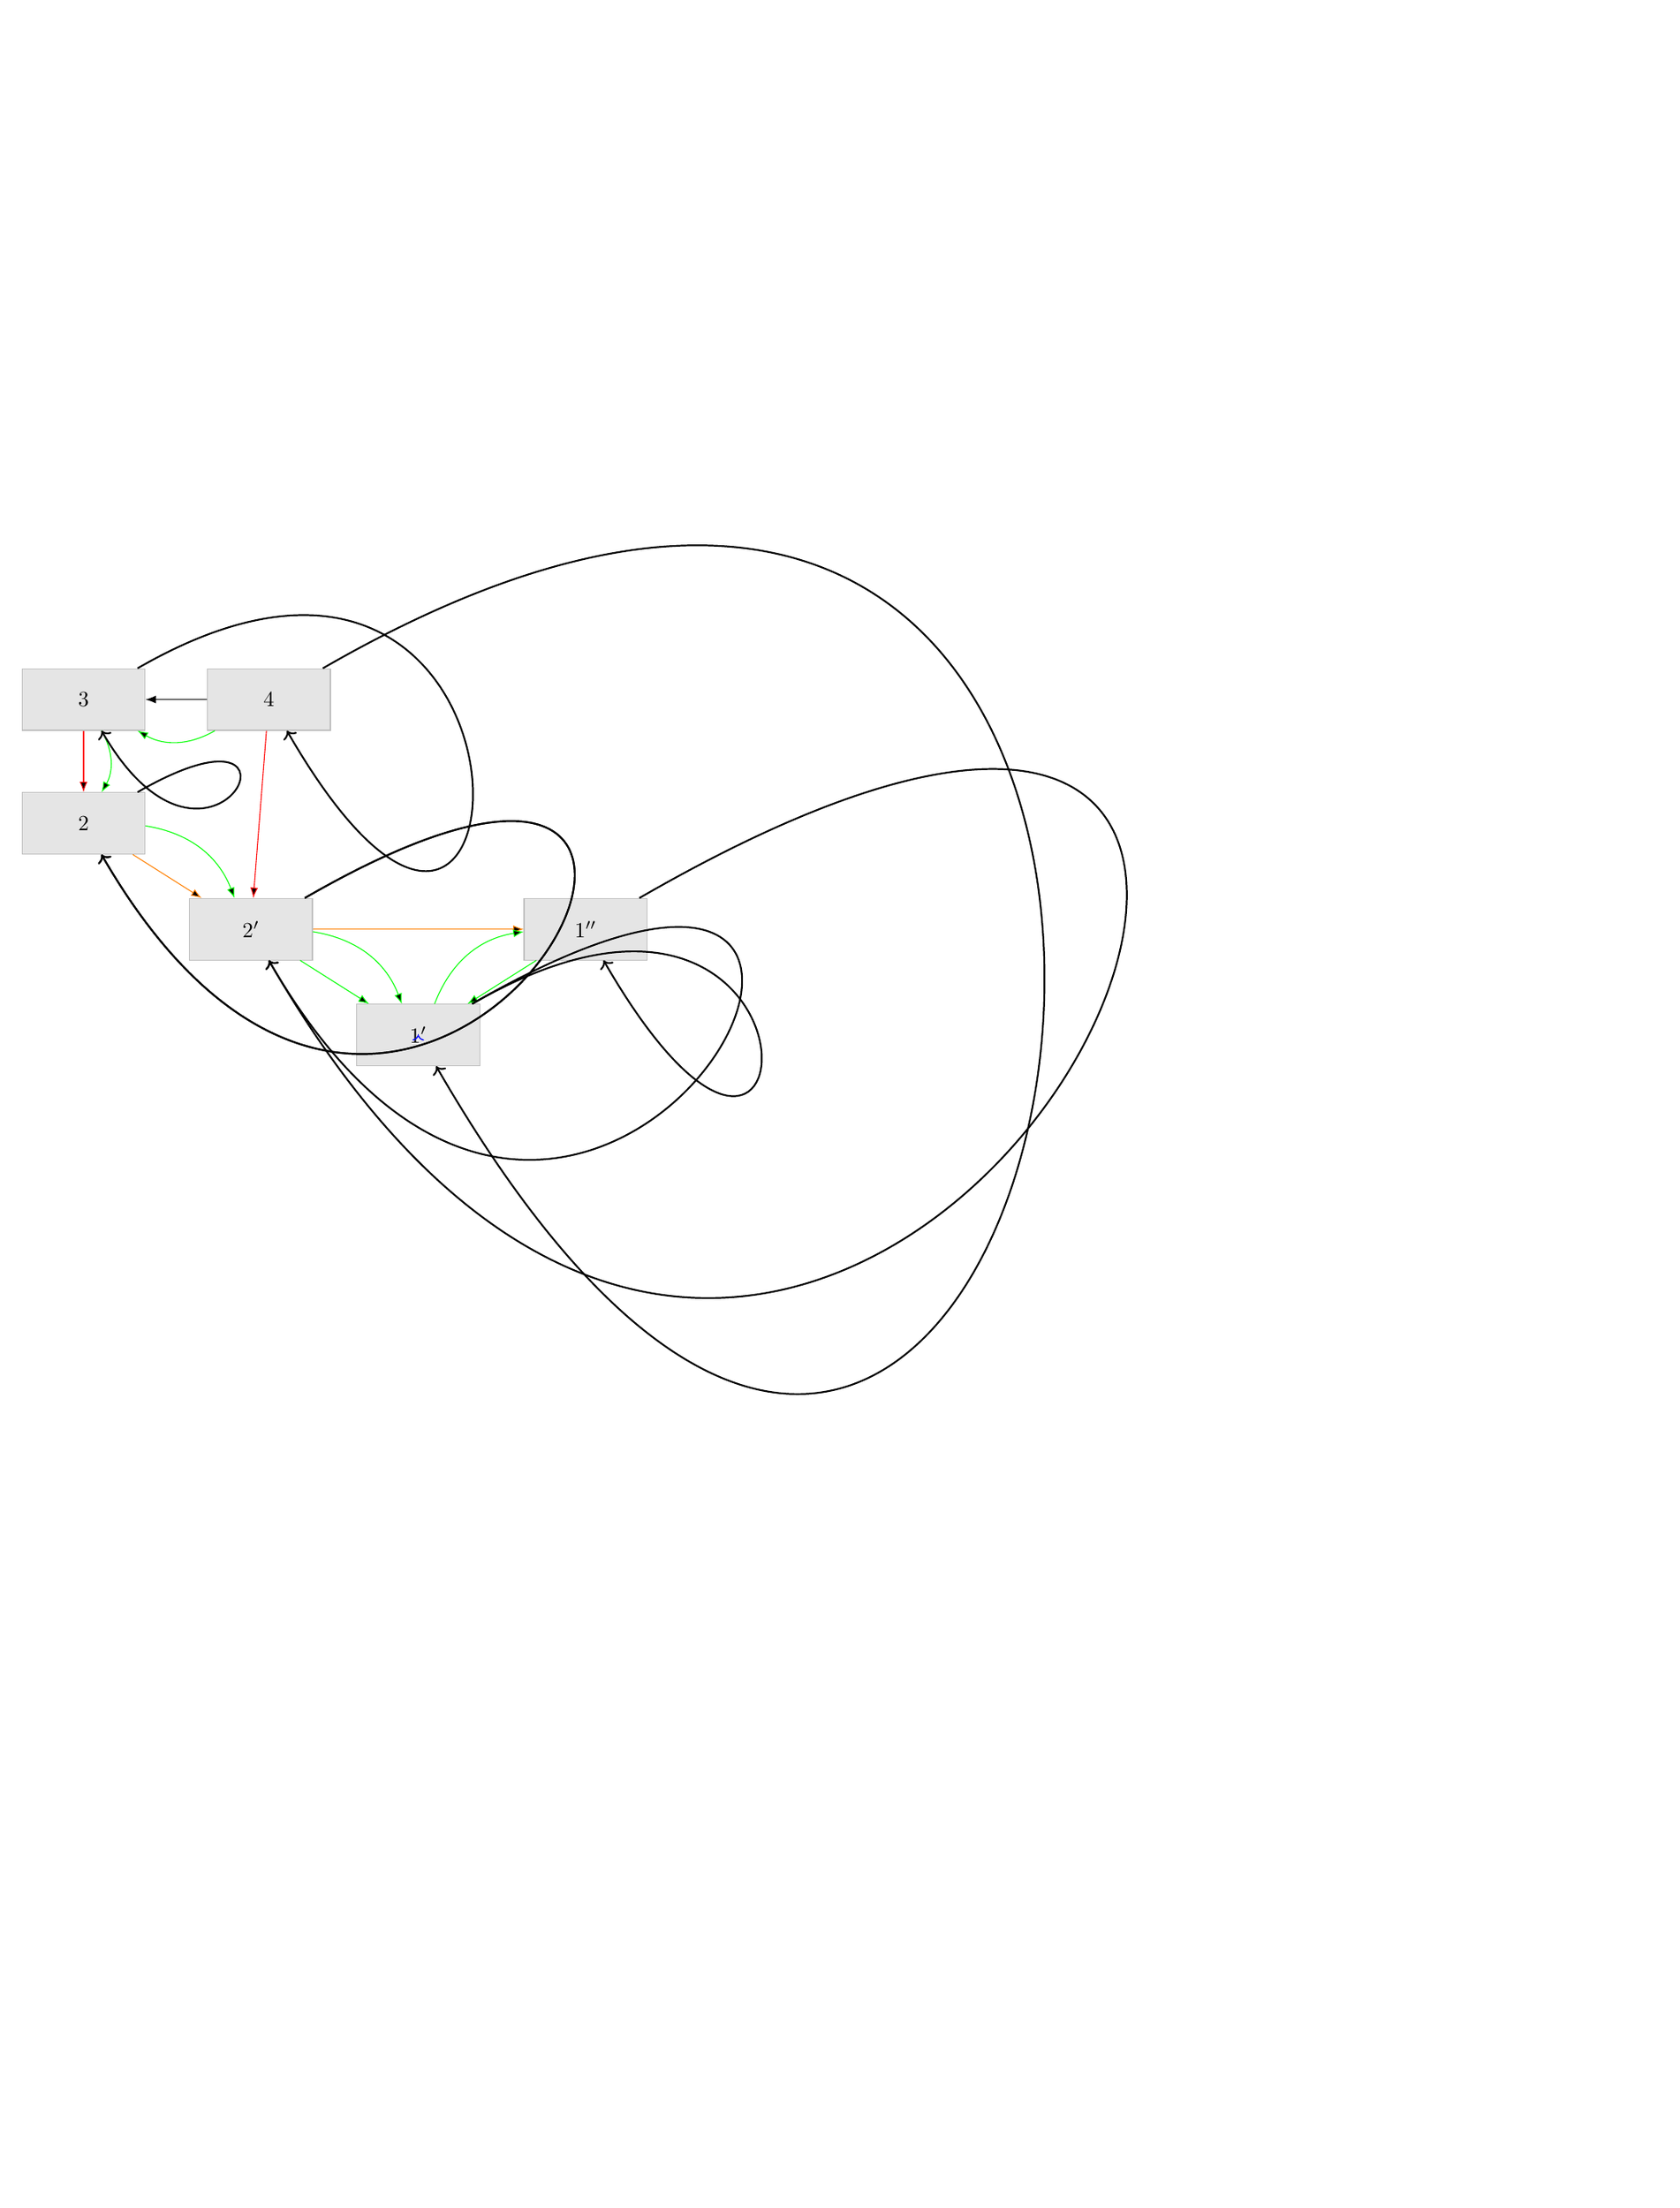
\begin{tikzpicture}[node distance=1cm,
    every node/.style={draw, minimum width=2cm, minimum height=1cm},
    buffer/.style={draw=gray!50, fill=gray!20},
    loop/.style={->, bend left=30, draw=blue},
    create/.style={->, draw=green, >=Latex},
    delete1/.style={->, draw=orange, >=Latex},
    delete2/.style={->, draw=red, >=Latex},
    delete3/.style={->, draw=black, >=Latex}]

  % Nodes
  \node (0) [buffer] {0};
  \node (1) [above left=of 0, buffer] {1};
  \node (2) [above left=of 1, buffer] {2};
  \node (3) [above=of 2, buffer] {3};
  \node (4) [right=of 3, buffer] {4};
  \node (1p) [below right=of 1, buffer] {$1'$};
  \node (1pp) [above right=of 1p, buffer] {$1''$};
  \node (2p) [below right=of 2, buffer] {$2'$};

  % Arrows
  \path[loop] (0) edge [looseness=8] (0);
  \path[create] (1) edge (0);
  \path[delete1] (2) edge (1);
  \path[delete2] (3) edge (2);
  \path[delete3] (4) edge (3);

  \path[loop] (1p) edge [looseness=8] (1p);
  \path[create] (1pp) edge (1p);
  \path[delete1] (2p) edge (1pp);
  \path[delete2] (4) edge (2p);

  % Additional arrows for the outer ring
  \path[create] (2) edge[bend left=30] (1);
  \path[create] (3) edge[bend left=30] (2);
  \path[create] (4) edge[bend left=30] (3);
  \path[create] (1p) edge[bend left=30] (1pp);
  \path[create] (2p) edge[bend left=30] (1p);

  % Outer ring
  \draw [thick, black, ->, looseness=8, out=30, in=-60] (0) to (1);
  \draw [thick, black, ->, looseness=8, out=30, in=-60] (1) to (2);
  \draw [thick, black, ->, looseness=8, out=30, in=-60] (2) to (3);
  \draw [thick, black, ->, looseness=8, out=30, in=-60] (3) to (4);
  \draw [thick, black, ->, looseness=8, out=30, in=-60] (4) to (1p);
  \draw [thick, black, ->, looseness=8, out=30, in=-60] (1p) to (1pp);
  \draw [thick, black, ->, looseness=8, out=30, in=-60] (1pp) to (2p);
  \draw [thick, black, ->, looseness=8, out=30, in=-60] (2p) to (2);

\end{tikzpicture}

\end{document}